% Generated by Sphinx.
\def\sphinxdocclass{report}
\documentclass[letterpaper,10pt,english]{sphinxmanual}
\usepackage[utf8]{inputenc}
\DeclareUnicodeCharacter{00A0}{\nobreakspace}
\usepackage{cmap}
\usepackage[T1]{fontenc}
\usepackage{babel}
\usepackage{times}
\usepackage[Bjarne]{fncychap}
\usepackage{longtable}
\usepackage{sphinx}
\usepackage{multirow}


\title{pyfluo Documentation}
\date{October 21, 2014}
\release{}
\author{Author}
\newcommand{\sphinxlogo}{}
\renewcommand{\releasename}{Release}
\makeindex

\makeatletter
\def\PYG@reset{\let\PYG@it=\relax \let\PYG@bf=\relax%
    \let\PYG@ul=\relax \let\PYG@tc=\relax%
    \let\PYG@bc=\relax \let\PYG@ff=\relax}
\def\PYG@tok#1{\csname PYG@tok@#1\endcsname}
\def\PYG@toks#1+{\ifx\relax#1\empty\else%
    \PYG@tok{#1}\expandafter\PYG@toks\fi}
\def\PYG@do#1{\PYG@bc{\PYG@tc{\PYG@ul{%
    \PYG@it{\PYG@bf{\PYG@ff{#1}}}}}}}
\def\PYG#1#2{\PYG@reset\PYG@toks#1+\relax+\PYG@do{#2}}

\expandafter\def\csname PYG@tok@gd\endcsname{\def\PYG@tc##1{\textcolor[rgb]{0.63,0.00,0.00}{##1}}}
\expandafter\def\csname PYG@tok@gu\endcsname{\let\PYG@bf=\textbf\def\PYG@tc##1{\textcolor[rgb]{0.50,0.00,0.50}{##1}}}
\expandafter\def\csname PYG@tok@gt\endcsname{\def\PYG@tc##1{\textcolor[rgb]{0.00,0.27,0.87}{##1}}}
\expandafter\def\csname PYG@tok@gs\endcsname{\let\PYG@bf=\textbf}
\expandafter\def\csname PYG@tok@gr\endcsname{\def\PYG@tc##1{\textcolor[rgb]{1.00,0.00,0.00}{##1}}}
\expandafter\def\csname PYG@tok@cm\endcsname{\let\PYG@it=\textit\def\PYG@tc##1{\textcolor[rgb]{0.25,0.50,0.56}{##1}}}
\expandafter\def\csname PYG@tok@vg\endcsname{\def\PYG@tc##1{\textcolor[rgb]{0.73,0.38,0.84}{##1}}}
\expandafter\def\csname PYG@tok@m\endcsname{\def\PYG@tc##1{\textcolor[rgb]{0.13,0.50,0.31}{##1}}}
\expandafter\def\csname PYG@tok@mh\endcsname{\def\PYG@tc##1{\textcolor[rgb]{0.13,0.50,0.31}{##1}}}
\expandafter\def\csname PYG@tok@cs\endcsname{\def\PYG@tc##1{\textcolor[rgb]{0.25,0.50,0.56}{##1}}\def\PYG@bc##1{\setlength{\fboxsep}{0pt}\colorbox[rgb]{1.00,0.94,0.94}{\strut ##1}}}
\expandafter\def\csname PYG@tok@ge\endcsname{\let\PYG@it=\textit}
\expandafter\def\csname PYG@tok@vc\endcsname{\def\PYG@tc##1{\textcolor[rgb]{0.73,0.38,0.84}{##1}}}
\expandafter\def\csname PYG@tok@il\endcsname{\def\PYG@tc##1{\textcolor[rgb]{0.13,0.50,0.31}{##1}}}
\expandafter\def\csname PYG@tok@go\endcsname{\def\PYG@tc##1{\textcolor[rgb]{0.20,0.20,0.20}{##1}}}
\expandafter\def\csname PYG@tok@cp\endcsname{\def\PYG@tc##1{\textcolor[rgb]{0.00,0.44,0.13}{##1}}}
\expandafter\def\csname PYG@tok@gi\endcsname{\def\PYG@tc##1{\textcolor[rgb]{0.00,0.63,0.00}{##1}}}
\expandafter\def\csname PYG@tok@gh\endcsname{\let\PYG@bf=\textbf\def\PYG@tc##1{\textcolor[rgb]{0.00,0.00,0.50}{##1}}}
\expandafter\def\csname PYG@tok@ni\endcsname{\let\PYG@bf=\textbf\def\PYG@tc##1{\textcolor[rgb]{0.84,0.33,0.22}{##1}}}
\expandafter\def\csname PYG@tok@nl\endcsname{\let\PYG@bf=\textbf\def\PYG@tc##1{\textcolor[rgb]{0.00,0.13,0.44}{##1}}}
\expandafter\def\csname PYG@tok@nn\endcsname{\let\PYG@bf=\textbf\def\PYG@tc##1{\textcolor[rgb]{0.05,0.52,0.71}{##1}}}
\expandafter\def\csname PYG@tok@no\endcsname{\def\PYG@tc##1{\textcolor[rgb]{0.38,0.68,0.84}{##1}}}
\expandafter\def\csname PYG@tok@na\endcsname{\def\PYG@tc##1{\textcolor[rgb]{0.25,0.44,0.63}{##1}}}
\expandafter\def\csname PYG@tok@nb\endcsname{\def\PYG@tc##1{\textcolor[rgb]{0.00,0.44,0.13}{##1}}}
\expandafter\def\csname PYG@tok@nc\endcsname{\let\PYG@bf=\textbf\def\PYG@tc##1{\textcolor[rgb]{0.05,0.52,0.71}{##1}}}
\expandafter\def\csname PYG@tok@nd\endcsname{\let\PYG@bf=\textbf\def\PYG@tc##1{\textcolor[rgb]{0.33,0.33,0.33}{##1}}}
\expandafter\def\csname PYG@tok@ne\endcsname{\def\PYG@tc##1{\textcolor[rgb]{0.00,0.44,0.13}{##1}}}
\expandafter\def\csname PYG@tok@nf\endcsname{\def\PYG@tc##1{\textcolor[rgb]{0.02,0.16,0.49}{##1}}}
\expandafter\def\csname PYG@tok@si\endcsname{\let\PYG@it=\textit\def\PYG@tc##1{\textcolor[rgb]{0.44,0.63,0.82}{##1}}}
\expandafter\def\csname PYG@tok@s2\endcsname{\def\PYG@tc##1{\textcolor[rgb]{0.25,0.44,0.63}{##1}}}
\expandafter\def\csname PYG@tok@vi\endcsname{\def\PYG@tc##1{\textcolor[rgb]{0.73,0.38,0.84}{##1}}}
\expandafter\def\csname PYG@tok@nt\endcsname{\let\PYG@bf=\textbf\def\PYG@tc##1{\textcolor[rgb]{0.02,0.16,0.45}{##1}}}
\expandafter\def\csname PYG@tok@nv\endcsname{\def\PYG@tc##1{\textcolor[rgb]{0.73,0.38,0.84}{##1}}}
\expandafter\def\csname PYG@tok@s1\endcsname{\def\PYG@tc##1{\textcolor[rgb]{0.25,0.44,0.63}{##1}}}
\expandafter\def\csname PYG@tok@gp\endcsname{\let\PYG@bf=\textbf\def\PYG@tc##1{\textcolor[rgb]{0.78,0.36,0.04}{##1}}}
\expandafter\def\csname PYG@tok@sh\endcsname{\def\PYG@tc##1{\textcolor[rgb]{0.25,0.44,0.63}{##1}}}
\expandafter\def\csname PYG@tok@ow\endcsname{\let\PYG@bf=\textbf\def\PYG@tc##1{\textcolor[rgb]{0.00,0.44,0.13}{##1}}}
\expandafter\def\csname PYG@tok@sx\endcsname{\def\PYG@tc##1{\textcolor[rgb]{0.78,0.36,0.04}{##1}}}
\expandafter\def\csname PYG@tok@bp\endcsname{\def\PYG@tc##1{\textcolor[rgb]{0.00,0.44,0.13}{##1}}}
\expandafter\def\csname PYG@tok@c1\endcsname{\let\PYG@it=\textit\def\PYG@tc##1{\textcolor[rgb]{0.25,0.50,0.56}{##1}}}
\expandafter\def\csname PYG@tok@kc\endcsname{\let\PYG@bf=\textbf\def\PYG@tc##1{\textcolor[rgb]{0.00,0.44,0.13}{##1}}}
\expandafter\def\csname PYG@tok@c\endcsname{\let\PYG@it=\textit\def\PYG@tc##1{\textcolor[rgb]{0.25,0.50,0.56}{##1}}}
\expandafter\def\csname PYG@tok@mf\endcsname{\def\PYG@tc##1{\textcolor[rgb]{0.13,0.50,0.31}{##1}}}
\expandafter\def\csname PYG@tok@err\endcsname{\def\PYG@bc##1{\setlength{\fboxsep}{0pt}\fcolorbox[rgb]{1.00,0.00,0.00}{1,1,1}{\strut ##1}}}
\expandafter\def\csname PYG@tok@kd\endcsname{\let\PYG@bf=\textbf\def\PYG@tc##1{\textcolor[rgb]{0.00,0.44,0.13}{##1}}}
\expandafter\def\csname PYG@tok@ss\endcsname{\def\PYG@tc##1{\textcolor[rgb]{0.32,0.47,0.09}{##1}}}
\expandafter\def\csname PYG@tok@sr\endcsname{\def\PYG@tc##1{\textcolor[rgb]{0.14,0.33,0.53}{##1}}}
\expandafter\def\csname PYG@tok@mo\endcsname{\def\PYG@tc##1{\textcolor[rgb]{0.13,0.50,0.31}{##1}}}
\expandafter\def\csname PYG@tok@mi\endcsname{\def\PYG@tc##1{\textcolor[rgb]{0.13,0.50,0.31}{##1}}}
\expandafter\def\csname PYG@tok@kn\endcsname{\let\PYG@bf=\textbf\def\PYG@tc##1{\textcolor[rgb]{0.00,0.44,0.13}{##1}}}
\expandafter\def\csname PYG@tok@o\endcsname{\def\PYG@tc##1{\textcolor[rgb]{0.40,0.40,0.40}{##1}}}
\expandafter\def\csname PYG@tok@kr\endcsname{\let\PYG@bf=\textbf\def\PYG@tc##1{\textcolor[rgb]{0.00,0.44,0.13}{##1}}}
\expandafter\def\csname PYG@tok@s\endcsname{\def\PYG@tc##1{\textcolor[rgb]{0.25,0.44,0.63}{##1}}}
\expandafter\def\csname PYG@tok@kp\endcsname{\def\PYG@tc##1{\textcolor[rgb]{0.00,0.44,0.13}{##1}}}
\expandafter\def\csname PYG@tok@w\endcsname{\def\PYG@tc##1{\textcolor[rgb]{0.73,0.73,0.73}{##1}}}
\expandafter\def\csname PYG@tok@kt\endcsname{\def\PYG@tc##1{\textcolor[rgb]{0.56,0.13,0.00}{##1}}}
\expandafter\def\csname PYG@tok@sc\endcsname{\def\PYG@tc##1{\textcolor[rgb]{0.25,0.44,0.63}{##1}}}
\expandafter\def\csname PYG@tok@sb\endcsname{\def\PYG@tc##1{\textcolor[rgb]{0.25,0.44,0.63}{##1}}}
\expandafter\def\csname PYG@tok@k\endcsname{\let\PYG@bf=\textbf\def\PYG@tc##1{\textcolor[rgb]{0.00,0.44,0.13}{##1}}}
\expandafter\def\csname PYG@tok@se\endcsname{\let\PYG@bf=\textbf\def\PYG@tc##1{\textcolor[rgb]{0.25,0.44,0.63}{##1}}}
\expandafter\def\csname PYG@tok@sd\endcsname{\let\PYG@it=\textit\def\PYG@tc##1{\textcolor[rgb]{0.25,0.44,0.63}{##1}}}

\def\PYGZbs{\char`\\}
\def\PYGZus{\char`\_}
\def\PYGZob{\char`\{}
\def\PYGZcb{\char`\}}
\def\PYGZca{\char`\^}
\def\PYGZam{\char`\&}
\def\PYGZlt{\char`\<}
\def\PYGZgt{\char`\>}
\def\PYGZsh{\char`\#}
\def\PYGZpc{\char`\%}
\def\PYGZdl{\char`\$}
\def\PYGZhy{\char`\-}
\def\PYGZsq{\char`\'}
\def\PYGZdq{\char`\"}
\def\PYGZti{\char`\~}
% for compatibility with earlier versions
\def\PYGZat{@}
\def\PYGZlb{[}
\def\PYGZrb{]}
\makeatother

\begin{document}

\maketitle
\tableofcontents
\phantomsection\label{index::doc}



\chapter{About this library}
\label{introduction:welcome-to-the-documentation-for-pyfluo}\label{introduction:about-this-library}\label{introduction::doc}
The \textbf{pyfluo} library enables easy and efficient manipulation of imaging data using a set of custom-built data structures and functions.

This project is \href{https://github.com/bensondaled/pyfluo/}{hosted on github}.

Note that \textbf{pyfluo} is a work in progress; neither the code nor the documentation is complete. That said, it is already functional for a wide variety of tasks.


\chapter{Requirements}
\label{introduction:requirements}
The library only depends upon the standard python library, plus Numpy, Scipy, and Matplotlib.


\chapter{Installation}
\label{introduction:installation}\begin{enumerate}
\item {} 
Download the project \href{https://github.com/bensondaled/pyfluo/}{here}.

\item {} 
Extract and navigate to the root directory.

\item {} 
Run \code{python setup.py install}

\end{enumerate}


\chapter{A quick example}
\label{introduction:a-quick-example}
Here is a quick-start example to get you moving with pyfluo.

\begin{Verbatim}[commandchars=\\\{\},numbers=left,firstnumber=1,stepnumber=1]
\PYG{k+kn}{from} \PYG{n+nn}{pyfluo} \PYG{k+kn}{import} \PYG{n}{MultiChannelTiff}\PYG{p}{,} \PYG{n}{Movie}\PYG{p}{,} \PYG{n}{LineScan}
\PYG{k+kn}{from} \PYG{n+nn}{pyfluo.fluorescence} \PYG{k+kn}{import} \PYG{n}{compute\PYGZus{}dff}
\PYG{k+kn}{from} \PYG{n+nn}{pyfluo.tiff} \PYG{k+kn}{import} \PYG{n}{CHANNEL\PYGZus{}IMG}\PYG{p}{,} \PYG{n}{CHANNEL\PYGZus{}STIM}
\PYG{k+kn}{from} \PYG{n+nn}{pyfluo.io} \PYG{k+kn}{import} \PYG{n}{save}\PYG{p}{,} \PYG{n}{load}
\PYG{k+kn}{import} \PYG{n+nn}{os}
\PYG{k+kn}{import} \PYG{n+nn}{numpy} \PYG{k+kn}{as} \PYG{n+nn}{np}
\PYG{k+kn}{import} \PYG{n+nn}{pylab} \PYG{k+kn}{as} \PYG{n+nn}{pl}
\PYG{n}{pl}\PYG{o}{.}\PYG{n}{ion}\PYG{p}{(}\PYG{p}{)}

\PYG{c}{\PYGZsh{} reload previously saved data}
\PYG{n+nb}{globals}\PYG{p}{(}\PYG{p}{)}\PYG{o}{.}\PYG{n}{update}\PYG{p}{(}\PYG{n}{load}\PYG{p}{(}\PYG{l+s}{\PYGZsq{}}\PYG{l+s}{my\PYGZus{}saved\PYGZus{}data}\PYG{l+s}{\PYGZsq{}}\PYG{p}{)}\PYG{p}{)}

\PYG{c}{\PYGZsh{} specify tif files to be loaded}
\PYG{n}{dir\PYGZus{}name} \PYG{o}{=} \PYG{l+s}{\PYGZsq{}}\PYG{l+s}{./lab\PYGZhy{}data/experiment\PYGZhy{}june25/}\PYG{l+s}{\PYGZsq{}}
\PYG{n}{names} \PYG{o}{=} \PYG{p}{[}\PYG{n}{os}\PYG{o}{.}\PYG{n}{path}\PYG{o}{.}\PYG{n}{join}\PYG{p}{(}\PYG{n}{dir\PYGZus{}name}\PYG{p}{,}\PYG{n}{file\PYGZus{}name}\PYG{p}{)} \PYG{k}{for} \PYG{n}{file\PYGZus{}name} \PYG{o+ow}{in} \PYG{n}{os}\PYG{o}{.}\PYG{n}{listdir}\PYG{p}{(}\PYG{n}{dir\PYGZus{}name}\PYG{p}{)} \PYG{k}{if} \PYG{l+s}{\PYGZsq{}}\PYG{l+s}{500Hz}\PYG{l+s}{\PYGZsq{}} \PYG{o+ow}{in} \PYG{n}{file\PYGZus{}name}\PYG{p}{]}

\PYG{c}{\PYGZsh{} load tif files}
\PYG{n}{mct} \PYG{o}{=} \PYG{n}{MultiChannelTiff}\PYG{p}{(}\PYG{n}{names}\PYG{p}{,} \PYG{n}{skip}\PYG{o}{=}\PYG{p}{(}\PYG{l+m+mi}{10}\PYG{p}{,}\PYG{l+m+mi}{0}\PYG{p}{,}\PYG{l+m+mi}{0}\PYG{p}{)}\PYG{p}{,} \PYG{n}{klass}\PYG{o}{=}\PYG{n}{Movie}\PYG{p}{)} \PYG{c}{\PYGZsh{} this skipped the first ten frames of each tiff file}
\PYG{c}{\PYGZsh{} mct = MultiChannelTiff(names, skip=(0,0,32), klass=LineScan) \PYGZsh{} this skipped every 32 lines in every tiff file}
\PYG{n}{mov} \PYG{o}{=} \PYG{n}{mct}\PYG{p}{[}\PYG{n}{CHANNEL\PYGZus{}IMG}\PYG{p}{]}
\PYG{n}{stim} \PYG{o}{=} \PYG{n}{mct}\PYG{p}{[}\PYG{n}{CHANNEL\PYGZus{}STIM}\PYG{p}{]}\PYG{o}{.}\PYG{n}{flatten}\PYG{p}{(}\PYG{p}{)}

\PYG{c}{\PYGZsh{} play the movie}
\PYG{n}{mov}\PYG{o}{.}\PYG{n}{play}\PYG{p}{(}\PYG{n}{fps}\PYG{o}{=}\PYG{l+m+mi}{15}\PYG{p}{)}

\PYG{c}{\PYGZsh{} extract and align stimulation events from movie, then play result}
\PYG{n}{mov\PYGZus{}stims} \PYG{o}{=} \PYG{n}{mov}\PYG{o}{.}\PYG{n}{take}\PYG{p}{(}\PYG{n}{stim}\PYG{o}{.}\PYG{n}{stim\PYGZus{}times}\PYG{p}{,} \PYG{n}{pad}\PYG{o}{=}\PYG{p}{(}\PYG{o}{.}\PYG{l+m+mi}{5}\PYG{p}{,} \PYG{o}{.}\PYG{l+m+mi}{5}\PYG{p}{)}\PYG{p}{,} \PYG{n}{merge\PYGZus{}method}\PYG{o}{=}\PYG{n}{np}\PYG{o}{.}\PYG{n}{mean}\PYG{p}{)}
\PYG{n}{mov\PYGZus{}stims}\PYG{o}{.}\PYG{n}{play}\PYG{p}{(}\PYG{n}{loop}\PYG{o}{=}\PYG{n+nb+bp}{True}\PYG{p}{)}

\PYG{c}{\PYGZsh{} select some regions of interest \PYGZam{} extract their signals}
\PYG{n}{mov}\PYG{o}{.}\PYG{n}{select\PYGZus{}roi}\PYG{p}{(}\PYG{l+m+mi}{3}\PYG{p}{)}
\PYG{n}{signals} \PYG{o}{=} \PYG{n}{mov}\PYG{o}{.}\PYG{n}{extract\PYGZus{}by\PYGZus{}roi}\PYG{p}{(}\PYG{p}{)}

\PYG{c}{\PYGZsh{} compute delta\PYGZhy{}f over f of signals}
\PYG{n}{dff} \PYG{o}{=} \PYG{n}{compute\PYGZus{}dff}\PYG{p}{(}\PYG{n}{signals}\PYG{p}{)}

\PYG{c}{\PYGZsh{} extract and align stimulation events from signals}
\PYG{n}{dff\PYGZus{}stims} \PYG{o}{=} \PYG{n}{dff}\PYG{o}{.}\PYG{n}{take}\PYG{p}{(}\PYG{n}{stim}\PYG{o}{.}\PYG{n}{stim\PYGZus{}times}\PYG{p}{,} \PYG{n}{pad}\PYG{o}{=}\PYG{p}{(}\PYG{o}{.}\PYG{l+m+mi}{5}\PYG{p}{,}\PYG{o}{.}\PYG{l+m+mi}{5}\PYG{p}{)}\PYG{p}{)}

\PYG{c}{\PYGZsh{} plot the result}
\PYG{n}{dff\PYGZus{}stims}\PYG{o}{.}\PYG{n}{plot}\PYG{p}{(}\PYG{n}{stim}\PYG{o}{=}\PYG{n}{stim}\PYG{o}{.}\PYG{n}{example}\PYG{p}{)}

\PYG{c}{\PYGZsh{} show the regions corresponding to plot}
\PYG{n}{pl}\PYG{o}{.}\PYG{n}{figure}\PYG{p}{(}\PYG{p}{)}
\PYG{n}{mov}\PYG{o}{.}\PYG{n}{z\PYGZus{}project}\PYG{p}{(}\PYG{n}{show}\PYG{o}{=}\PYG{n+nb+bp}{True}\PYG{p}{,} \PYG{n}{rois}\PYG{o}{=}\PYG{n+nb+bp}{True}\PYG{p}{)}

\PYG{c}{\PYGZsh{} save the figures}
\PYG{n}{pl}\PYG{o}{.}\PYG{n}{savefig}\PYG{p}{(}\PYG{l+s}{\PYGZsq{}}\PYG{l+s}{rois.png}\PYG{l+s}{\PYGZsq{}}\PYG{p}{)}
\PYG{n}{pl}\PYG{o}{.}\PYG{n}{figure}\PYG{p}{(}\PYG{l+m+mi}{1}\PYG{p}{)}
\PYG{n}{pl}\PYG{o}{.}\PYG{n}{savefig}\PYG{p}{(}\PYG{l+s}{\PYGZsq{}}\PYG{l+s}{dff\PYGZus{}aligned.png}\PYG{l+s}{\PYGZsq{}}\PYG{p}{)}
\PYG{c}{\PYGZsh{} and the data}
\PYG{n}{save}\PYG{p}{(}\PYG{l+s}{\PYGZsq{}}\PYG{l+s}{my\PYGZus{}new\PYGZus{}data}\PYG{l+s}{\PYGZsq{}}\PYG{p}{,} \PYG{n}{dff}\PYG{o}{=}\PYG{n}{dff}\PYG{p}{,} \PYG{n}{stim}\PYG{o}{=}\PYG{n}{stim}\PYG{p}{)}
\end{Verbatim}

Shown below are examples of rois.png (left) and dff\_aligned.png (right).

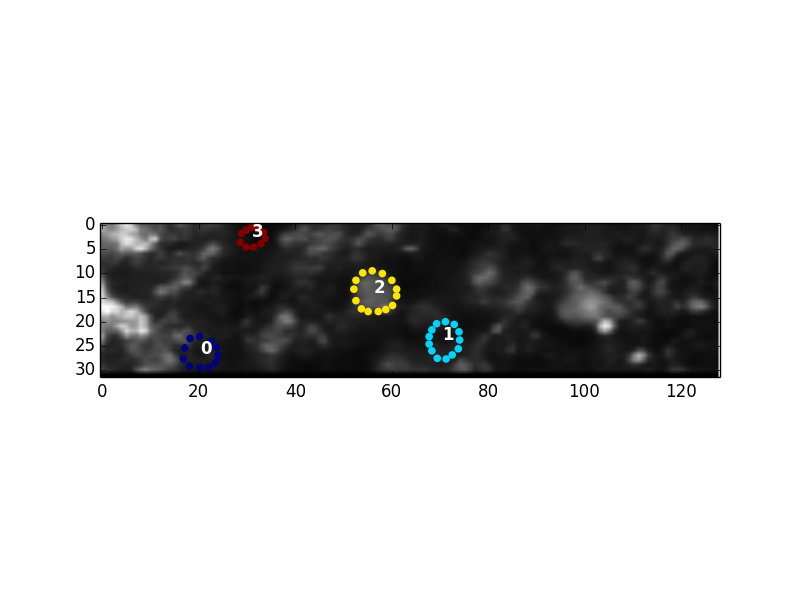
\includegraphics[width=0.400\linewidth]{rois.png}

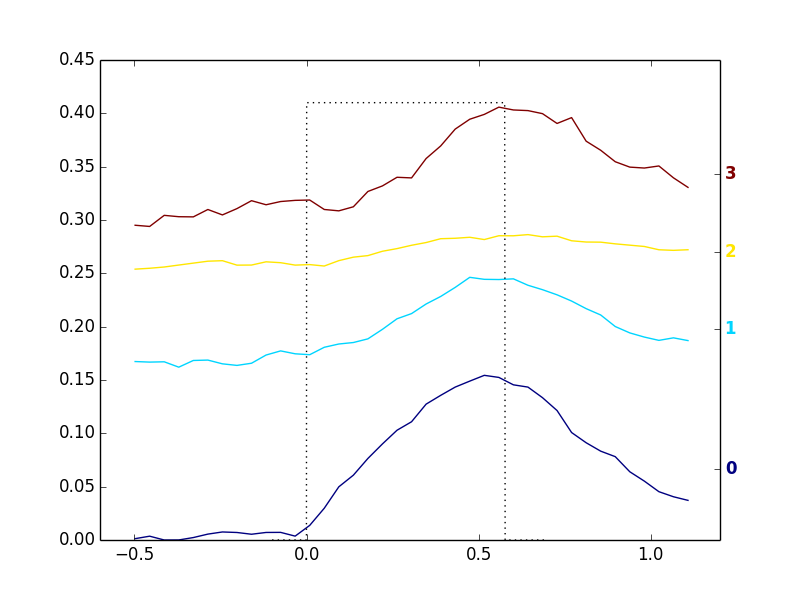
\includegraphics[width=0.400\linewidth]{dff_aligned.png}


\chapter{Troubleshooting}
\label{introduction:troubleshooting}
A list of known fixes for common problems will be kept here.
\begin{itemize}
\item {} 
For windows installations, VisualStudio often causes problems in installing the tiff module. A fix is explained \href{http://stackoverflow.com/questions/2817869/error-unable-to-find-vcvarsall-bat}{here}.

\end{itemize}


\chapter{Core Data Structures}
\label{data_structures::doc}\label{data_structures:core-data-structures}
\begin{longtable}{ll}
\hline
\endfirsthead

\multicolumn{2}{c}%
{{\textsf{\tablename\ \thetable{} -- continued from previous page}}} \\
\hline
\endhead

\hline \multicolumn{2}{|r|}{{\textsf{Continued on next page}}} \\ \hline
\endfoot

\endlastfoot


{\hyperref[data_structures:time_series.TimeSeries]{\code{time\_series.TimeSeries}}}(data{[}, time, info, ...{]})
 & 
A data structure that holds a one or more one-dimensional arrays of values, associated with a single time vector.
\\

{\hyperref[data_structures:stimulation.StimSeries]{\code{stimulation.StimSeries}}}(*args, **kwargs)
 & 
A time series specialized for storing stimulation data.
\\

{\hyperref[data_structures:tiff.wanglab.MultiChannelTiff]{\code{tiff.wanglab.MultiChannelTiff}}}(raw{[}, klass{]})
 & 
An object that holds multiple movie-like (from movies module) objects as channels.
\\

{\hyperref[data_structures:movies.Movie]{\code{movies.Movie}}}(data{[}, time, info, skip{]})
 & 
An object that holds a movie: a series of images each with a timestamp.
\\

{\hyperref[data_structures:movies.LineScan]{\code{movies.LineScan}}}(*args, **kwargs)
 & 
An object that holds a line scan:  a series of 1-dimensional images each with a timestamp.
\\
\hline\end{longtable}



\section{TimeSeries}
\label{data_structures:timeseries}\index{TimeSeries (class in time\_series)}

\begin{fulllineitems}
\phantomsection\label{data_structures:time_series.TimeSeries}\pysiglinewithargsret{\strong{class }\code{time\_series.}\bfcode{TimeSeries}}{\emph{data}, \emph{time=None}, \emph{info=None}, \emph{tunit='s'}, \emph{merge\_method\_data=\textless{}function mean at 0x10305d320\textgreater{}}, \emph{merge\_method\_time=\textless{}function mean at 0x10305d320\textgreater{}}}{}
A data structure that holds a one or more one-dimensional arrays of values, associated with a single time vector.

Note that because this object can store multiple data arrays as separate {\color{red}\bfseries{}{}`{}`}series'`, most of its methods perform operations in a parallel manner on each series. Unless otherwise noted, this is the default action of the class methods.
\begin{description}
\item[{\textbf{Attributes:}}] \leavevmode\begin{itemize}
\item {} 
\textbf{data} (\emph{np.ndarray}): the data array of the time series.

\item {} 
\textbf{time} (\emph{np.ndarray}): the time array of the time series.

\item {} 
\textbf{info} (\emph{np.ndarray}): an array of meta-information associated with time points.

\item {} 
\textbf{n\_series} (\emph{int}): the number of time series stored in the object (i.e. the number of rows in \emph{data}).

\item {} 
\textbf{Ts} (\emph{float}): the sampling period of the time series.

\item {} 
\textbf{fs} (\emph{float}): the sampling frequency of the time series.

\item {} 
\textbf{tunit} (\emph{str}): the unit of measurement in which the object's time is stored.

\item {} 
\textbf{name} (\emph{str}): a unique name generated for the object when instantiated

\end{itemize}

\item[{\textbf{Parameters:}}] \leavevmode\begin{itemize}
\item {} 
\textbf{data} (\emph{list} / \emph{np.ndarray} / \emph{TimeSeries}): the time series data. If type \emph{TimeSeries}, the \emph{time} parameter is ignored and time attribute from this parameter is used. See below for details on parameter format.

\item {} 
\textbf{time} (\emph{list} / \emph{np.ndarray}): list of uniformly spaced numerical values, identical in length to the number of columns in \emph{data}. If \emph{data} is type \emph{TimeSeries}, this parameter is ignored. If \code{None}, defaults to \code{range(len(data))}.

\item {} 
\textbf{info} (\emph{list} / \emph{np.ndarray}): list of meta-information associated with each time point.

\item {} 
\textbf{tunit} (\emph{str}): the unit of measurement in which the object's time is stored.

\item {} 
\textbf{merge\_method\_time} (\emph{def}): the function to be used to merge time vector when necessary. See notes on \emph{data} parameter for details.

\item {} 
\textbf{merge\_method\_data} (\emph{def}): the function to be used to merge the data vector when necessary. See notes on \emph{data} parameter for details.

\end{itemize}

\item[{\textbf{Notes:}}] \leavevmode
For the \emph{data} parameter, the only strict constraint is that all input contains the same number of samples. There are multple types of input that are supported:
\begin{enumerate}
\item {} 
The data of one or multiple time series. In the case of multiple time series, supply a list of lists, where each list is one of the time series. This can also be a 2D np.ndarray of the same structure. For example:

\begin{Verbatim}[commandchars=\\\{\}]
\PYG{g+gp}{\PYGZgt{}\PYGZgt{}\PYGZgt{} }\PYG{n}{data} \PYG{o}{=} \PYG{p}{[} \PYG{l+m+mf}{31.6}\PYG{p}{,} \PYG{l+m+mf}{81.5}\PYG{p}{,} \PYG{l+m+mf}{51.8}\PYG{p}{,} \PYG{l+m+mf}{93.7}\PYG{p}{,} \PYG{l+m+mf}{12.2}\PYG{p}{,} \PYG{l+m+mf}{16.1} \PYG{p}{]}   
\PYG{g+go}{            }
\PYG{g+gp}{\PYGZgt{}\PYGZgt{}\PYGZgt{} }\PYG{n}{data} \PYG{o}{=} \PYG{p}{[} \PYG{p}{[}\PYG{l+m+mf}{5.5}\PYG{p}{,} \PYG{l+m+mf}{6.1}\PYG{p}{,} \PYG{l+m+mf}{3.3}\PYG{p}{]}\PYG{p}{,}
\PYG{g+gp}{\PYGZgt{}\PYGZgt{}\PYGZgt{} }         \PYG{p}{[}\PYG{l+m+mf}{2.8}\PYG{p}{,} \PYG{l+m+mf}{1.6}\PYG{p}{,} \PYG{l+m+mf}{9.8}\PYG{p}{]}\PYG{p}{,}
\PYG{g+gp}{\PYGZgt{}\PYGZgt{}\PYGZgt{} }         \PYG{p}{[}\PYG{l+m+mf}{1.2}\PYG{p}{,} \PYG{l+m+mf}{3.4}\PYG{p}{,} \PYG{l+m+mf}{5.2}\PYG{p}{]} \PYG{p}{]}
\end{Verbatim}

\item {} 
A list of TimeSeries objects. This situation is handled in various ways depending on the nature of the input:
\begin{quote}

\textbf{(a)} If the supplied TimeSeries objects all contain just single time series (i.e. \code{TimeSeries.n\_series == 1}), they are concatenated and the resulting TimeSeries will contain multiple rows of data corresponding to those inputs. The time vectors of the series are merged using the function given by the \emph{merge\_method\_time} argument in the constructor.

\textbf{(b)} If the supplied TimeSeries objects contain varying numbers of time series (i.e. \code{TimeSeries.n\_series} varies), the course of action is the same as (a), concatenating all the series from each TimeSeries object into one large TimeSeries object. Again, time vectors are merged as in (a).

\textbf{(c)} If the supplied TimeSeries objects contain multiple time series (i.e. two-dimensional data vectors), and \emph{every one has the same number of series}, it is assumed that there is a relationship between the series, and they are merged. Specifically, the first series (or data row) from every supplied TimeSeries is merged into one, then the second, then third, etc. The merge is performed by the \emph{merge\_method\_data} constructor argument. This course of action can be overridden by setting the \emph{merge\_method\_data} constructor argument to None, in which case the input will be handled as in (b).
\end{quote}

\end{enumerate}

\item[{\textbf{Usage Tips:}}] \leavevmode
The \emph{TimeSeries} object is in many ways like a numpy ndarray. In general it is safe to assume that operations performed on the object will be performed on the \emph{data} attribute. Here are some basic pointers for using \emph{TimeSeries}:
\begin{itemize}
\item {} 
Indexing:

\begin{Verbatim}[commandchars=\\\{\}]
\# create a time series
\textgreater{}\textgreater{}\textgreater{} ts = TimeSeries(data = [2.0, 4.0, 8.0, 16.0, 32.0])

\# basic indexing
\textgreater{}\textgreater{}\textgreater{} ts[0]
2.0

\# slicing
\textgreater{}\textgreater{}\textgreater{} ts[2:4]
np.array([8.0, 16.0])

\# create a TimeSeries with multiple series
\textgreater{}\textgreater{}\textgreater{} ts = TimeSeries(data = [ [2.0, 4.0, 6.0],
\textgreater{}\textgreater{}\textgreater{}                          [1.0, 2.0, 3.0],
\textgreater{}\textgreater{}\textgreater{}                          [5.0, 10.0, 15.0] ])

\# regular indexing
\textgreater{}\textgreater{}\textgreater{} ts[1]
np.array([ 4.0,
           2.0,
           10.0 ])

\# index a series using a string
\textgreater{}\textgreater{}\textgreater{} ts['1']
TimeSeries(data: [1.0, 2.0, 3.0])
\end{Verbatim}

\item {} 
Arithmetic:

\begin{Verbatim}[commandchars=\\\{\}]
\# create some time series
\textgreater{}\textgreater{}\textgreater{} ts1 = TimeSeries(data = [2.0, 4.0, 8.0, 16.0])
\textgreater{}\textgreater{}\textgreater{} ts2 = TimeSeries(data = [10.0, 20.0, 30.0, 40.0])

\# add TimeSeries
\textgreater{}\textgreater{}\textgreater{} ts1 + ts2
TimeSeries(data: [12.0, 24.0, 38.0 56.0])
\end{Verbatim}

\end{itemize}

\end{description}
\index{append() (time\_series.TimeSeries method)}

\begin{fulllineitems}
\phantomsection\label{data_structures:time_series.TimeSeries.append}\pysiglinewithargsret{\bfcode{append}}{\emph{item}}{}
Append data to the series.
\begin{description}
\item[{\textbf{Parameters:}}] \leavevmode\begin{itemize}
\item {} 
\textbf{item} (\emph{int} / \emph{float} / \emph{np.ndarray} / \emph{list}): the data to be appended to the series.

\end{itemize}

If a single value is supplied, the value is added to the end of the data. In the case that multiple data rows already exist in the data, the new entry is added to the end of each series.
If a list or array is supplied, it must be the same length as the number of series (i.e. rows of data) in the object's data. In this case, the first item in the list is added to the end of the first series, the second to the second, and so on.

\end{description}

Examples:

\begin{Verbatim}[commandchars=\\\{\}]
\# example 1

\textgreater{}\textgreater{}\textgreater{} ts.data = [ [1, 2, 3],
\textgreater{}\textgreater{}\textgreater{}             [4, 5, 6],
\textgreater{}\textgreater{}\textgreater{}             [7, 8, 9] ]
 
\textgreater{}\textgreater{}\textgreater{} ts.append(42)
 
\textgreater{}\textgreater{}\textgreater{} ts.data

[ [1, 2, 3, 42],
  [4, 5, 6, 42],
  [7, 8, 9, 42] ]

\# example 2
        
\textgreater{}\textgreater{}\textgreater{} ts.data = [ [1, 2],
\textgreater{}\textgreater{}\textgreater{}             [3, 4],
\textgreater{}\textgreater{}\textgreater{}             [5, 6] ]
        
\textgreater{}\textgreater{}\textgreater{} ts.append([66, 77, 88])

\textgreater{}\textgreater{}\textgreater{} ts.data

[ [1, 2, 66],
  [3, 4, 77],
  [5, 6, 88] ]
\end{Verbatim}

\end{fulllineitems}

\index{append\_series() (time\_series.TimeSeries method)}

\begin{fulllineitems}
\phantomsection\label{data_structures:time_series.TimeSeries.append_series}\pysiglinewithargsret{\bfcode{append\_series}}{\emph{item}, \emph{merge\_method\_time=\textless{}function mean at 0x10305d320\textgreater{}}}{}
Append a series, or row of data, to the object.
\begin{description}
\item[{\textbf{Parameters:}}] \leavevmode\begin{itemize}
\item {} 
\textbf{item} (\emph{np.ndarray} / \emph{list} / \emph{TimeSeries}): array of data to be added as a new row, or series. This must be the same length as the number of time points (i.e. columns) in the object's data.

\item {} 
\textbf{merge\_method\_time} (\emph{def}): function to be used to merge time vectors (applies when \emph{item} is a \emph{TimeSeries}).

\end{itemize}

\end{description}

Example:

\begin{Verbatim}[commandchars=\\\{\}]
\PYG{g+gp}{\PYGZgt{}\PYGZgt{}\PYGZgt{} }\PYG{n}{ts}\PYG{o}{.}\PYG{n}{data} \PYG{o}{=} \PYG{p}{[} \PYG{p}{[}\PYG{l+m+mi}{1}\PYG{p}{,} \PYG{l+m+mi}{2}\PYG{p}{,} \PYG{l+m+mi}{3}\PYG{p}{]}\PYG{p}{,}
\PYG{g+gp}{\PYGZgt{}\PYGZgt{}\PYGZgt{} }            \PYG{p}{[}\PYG{l+m+mi}{4}\PYG{p}{,} \PYG{l+m+mi}{5}\PYG{p}{,} \PYG{l+m+mi}{6}\PYG{p}{]}\PYG{p}{,}
\PYG{g+gp}{\PYGZgt{}\PYGZgt{}\PYGZgt{} }            \PYG{p}{[}\PYG{l+m+mi}{7}\PYG{p}{,} \PYG{l+m+mi}{8}\PYG{p}{,} \PYG{l+m+mi}{9}\PYG{p}{]} \PYG{p}{]}
\PYG{g+go}{        }
\PYG{g+gp}{\PYGZgt{}\PYGZgt{}\PYGZgt{} }\PYG{n}{ts}\PYG{o}{.}\PYG{n}{append\PYGZus{}series}\PYG{p}{(}\PYG{p}{[}\PYG{l+m+mi}{10}\PYG{p}{,} \PYG{l+m+mi}{11}\PYG{p}{,} \PYG{l+m+mi}{12}\PYG{p}{]}\PYG{p}{)}

\PYG{g+gp}{\PYGZgt{}\PYGZgt{}\PYGZgt{} }\PYG{n}{ts}\PYG{o}{.}\PYG{n}{data} 

\PYG{g+go}{[ [1, 2, 3],}
\PYG{g+go}{  [4, 5, 6],}
\PYG{g+go}{  [7, 8, 9],    }
\PYG{g+go}{  [10, 11, 12] ]}
\end{Verbatim}

\end{fulllineitems}

\index{get\_series() (time\_series.TimeSeries method)}

\begin{fulllineitems}
\phantomsection\label{data_structures:time_series.TimeSeries.get_series}\pysiglinewithargsret{\bfcode{get\_series}}{\emph{idx}}{}
Get one row of data (one series).
\begin{description}
\item[{\textbf{Parameters:}}] \leavevmode\begin{itemize}
\item {} 
\textbf{idx} (\emph{int}): the index of the desired series (i.e. row of data).

\end{itemize}

\item[{\textbf{Returns:}}] \leavevmode
A TimeSeries object.

\end{description}

\begin{notice}{note}{Note:}
Note that this is equivalent to the simpler string-based indexing. For example, \code{ts.get\_series(1)} is equivalent to \code{ts{[}'1'{]}}.
\end{notice}

\end{fulllineitems}

\index{merge() (time\_series.TimeSeries method)}

\begin{fulllineitems}
\phantomsection\label{data_structures:time_series.TimeSeries.merge}\pysiglinewithargsret{\bfcode{merge}}{\emph{method=\textless{}function mean at 0x10305d320\textgreater{}}}{}
Merge the series (data rows) of the object.
\begin{description}
\item[{\textbf{Parameters:}}] \leavevmode\begin{itemize}
\item {} 
\textbf{method} (\emph{def}): the function with which to perform the merge.

\end{itemize}

\item[{\textbf{Returns:}}] \leavevmode
A new \emph{TimeSeries} object with just one row of data, the merged result.

\end{description}

Example:

\begin{Verbatim}[commandchars=\\\{\}]
\PYG{g+gp}{\PYGZgt{}\PYGZgt{}\PYGZgt{} }\PYG{n}{ts}\PYG{o}{.}\PYG{n}{data} \PYG{o}{=} \PYG{p}{[} \PYG{p}{[}\PYG{l+m+mi}{1}\PYG{p}{,} \PYG{l+m+mi}{3}\PYG{p}{,} \PYG{l+m+mi}{5}\PYG{p}{]}\PYG{p}{,}
\PYG{g+gp}{\PYGZgt{}\PYGZgt{}\PYGZgt{} }            \PYG{p}{[}\PYG{l+m+mi}{2}\PYG{p}{,} \PYG{l+m+mi}{4}\PYG{p}{,} \PYG{l+m+mi}{6}\PYG{p}{]}\PYG{p}{,}
\PYG{g+gp}{\PYGZgt{}\PYGZgt{}\PYGZgt{} }            \PYG{p}{[}\PYG{l+m+mi}{9}\PYG{p}{,} \PYG{l+m+mi}{2}\PYG{p}{,} \PYG{l+m+mi}{7}\PYG{p}{]} \PYG{p}{]}

\PYG{g+gp}{\PYGZgt{}\PYGZgt{}\PYGZgt{} }\PYG{n}{ts} \PYG{o}{=} \PYG{n}{ts}\PYG{o}{.}\PYG{n}{merge}\PYG{p}{(}\PYG{n}{method}\PYG{o}{=}\PYG{n}{np}\PYG{o}{.}\PYG{n}{mean}\PYG{p}{)}

\PYG{g+gp}{\PYGZgt{}\PYGZgt{}\PYGZgt{} }\PYG{n}{ts}\PYG{o}{.}\PYG{n}{data}

\PYG{g+go}{[ [4, 3, 6] ]}
\end{Verbatim}

\end{fulllineitems}

\index{normalize() (time\_series.TimeSeries method)}

\begin{fulllineitems}
\phantomsection\label{data_structures:time_series.TimeSeries.normalize}\pysiglinewithargsret{\bfcode{normalize}}{\emph{minmax=(0.0}, \emph{1.0)}, \emph{by\_series=True}, \emph{in\_place=False}}{}
Normalize the time series object.
\begin{description}
\item[{\textbf{Parameters:}}] \leavevmode\begin{itemize}
\item {} 
\textbf{minmax} (\emph{list}): \code{{[}post\_normalizaton\_data\_min, max{]}}

\item {} 
\textbf{by\_series} (\emph{bool}): normalize each data row individually

\item {} 
\textbf{in\_place}: apply the normalization to \emph{this} instance of the object.

\end{itemize}

\item[{\textbf{Returns:}}] \leavevmode
A new \emph{TimeSeries} object, normalized.

\end{description}

Example:

\begin{Verbatim}[commandchars=\\\{\}]
\PYG{g+gp}{\PYGZgt{}\PYGZgt{}\PYGZgt{} }\PYG{n}{ts}\PYG{o}{.}\PYG{n}{data} \PYG{o}{=} \PYG{p}{[} \PYG{p}{[}\PYG{l+m+mi}{1}\PYG{p}{,} \PYG{l+m+mi}{2}\PYG{p}{,} \PYG{l+m+mi}{3}\PYG{p}{]}\PYG{p}{,}
\PYG{g+gp}{\PYGZgt{}\PYGZgt{}\PYGZgt{} }            \PYG{p}{[}\PYG{l+m+mi}{4}\PYG{p}{,} \PYG{l+m+mi}{5}\PYG{p}{,} \PYG{l+m+mi}{6}\PYG{p}{]}\PYG{p}{,}
\PYG{g+gp}{\PYGZgt{}\PYGZgt{}\PYGZgt{} }            \PYG{p}{[}\PYG{l+m+mi}{7}\PYG{p}{,} \PYG{l+m+mi}{8}\PYG{p}{,} \PYG{l+m+mi}{9}\PYG{p}{]} \PYG{p}{]}

\PYG{g+gp}{\PYGZgt{}\PYGZgt{}\PYGZgt{} }\PYG{n}{ts}\PYG{o}{.}\PYG{n}{normalize}\PYG{p}{(}\PYG{p}{)}

\PYG{g+gp}{\PYGZgt{}\PYGZgt{}\PYGZgt{} }\PYG{n}{ts}\PYG{o}{.}\PYG{n}{data}

\PYG{g+go}{[ [0, 0.5, 1],}
\PYG{g+go}{  [0, 0.5, 1],}
\PYG{g+go}{  [0, 0.5, 1] ]}
\end{Verbatim}

\end{fulllineitems}

\index{plot() (time\_series.TimeSeries method)}

\begin{fulllineitems}
\phantomsection\label{data_structures:time_series.TimeSeries.plot}\pysiglinewithargsret{\bfcode{plot}}{\emph{stim=None}, \emph{stacked=True}, \emph{gap\_fraction=0.08}, \emph{use\_idxs=False}, \emph{normalize=False}, \emph{show=True}, \emph{color=None}, \emph{**kwargs}}{}
Plot the time series.
\begin{description}
\item[{\textbf{Parameters:}}] \leavevmode\begin{itemize}
\item {} 
\textbf{stim} (\emph{pyfluo.StimSeries}): stimulation to be plotted over the data.

\item {} 
\textbf{stacked} (\emph{bool}): for multiple rows of data, stack instead of overlaying.

\item {} 
\textbf{gap\_fraction} (\emph{float}): if \code{stacked==True}, specifies the spacing between curves as a fraction of the average range of the curves.

\item {} 
\textbf{use\_idxs} (\emph{bool}): ignore time and instead use vector indices as x coordinate.

\item {} 
\textbf{normalize} (\emph{bool}): normalize the data before plotting.

\item {} 
\textbf{show} (\emph{bool}): show the plot immediately.

\item {} 
** \textbf{kwargs:} any arguments accepted by \emph{matplotlib.plot}

\end{itemize}

\end{description}

\end{fulllineitems}

\index{take() (time\_series.TimeSeries method)}

\begin{fulllineitems}
\phantomsection\label{data_structures:time_series.TimeSeries.take}\pysiglinewithargsret{\bfcode{take}}{\emph{time\_range}, \emph{pad=(0.0}, \emph{0.0)}, \emph{reset\_time=True}, \emph{merge\_method\_time=\textless{}function mean at 0x10305d320\textgreater{}}, \emph{merge\_method\_data=\textless{}function mean at 0x10305d320\textgreater{}}, \emph{**kwargs}}{}
Extract a range of data values using time indices.
\begin{description}
\item[{\textbf{Parameters:}}] \leavevmode\begin{itemize}
\item {} 
\textbf{time\_range} (\emph{list}): \code{{[}start\_time, end\_time{]}}

\item {} 
\textbf{pad} (\emph{list}): used optionally to expand the specified time range on either end. The first value is subtracted from the start time, and the second value is added to the end time.

\item {} 
\textbf{reset\_time} (\emph{bool}): shift the time vector of the resultant time series, such that time zero corresponds to the data originally located at \code{time\_range{[}0{]}}.

\item {} 
\textbf{merge\_method\_time} (\emph{def}): specifies how to merge time when multiple time ranges are extracted from multiple data series. See note below for details.

\item {} 
\textbf{merge\_method\_data} (\emph{def}): specifies how to merge data when multiple time ranges are extracted from multiple data series. See note below for details.

\end{itemize}

\item[{\textbf{Returns:}}] \leavevmode
A new \emph{TimeSeries} object with data corresponding to desired time range.

\item[{\textbf{Notes:}}] \leavevmode\begin{itemize}
\item {} 
The \emph{time\_range} parameter can be either a pair of values \code{(start\_time, end\_time)}, or a list of such pairs. In the latter case, this method is applied to each pair of times, and the result is a \emph{TimeSeries} object with multiple rows of data.

\item {} 
If values in \emph{time\_range} lie outside the bounds of the time series, or if the padding causes this to be true, the time vector is extrapolated accordingly, and the data for all non-existent points is given as \code{None}.

\item {} \begin{description}
\item[{Concerning merging of data: this method first extracts the desired time range/s from each row individually. If the original object contains multiple rows of data, there are two different results that should be expected: }] \leavevmode\begin{enumerate}
\item {} 
If only one time range is supplied, the resulting TimeSeries then contains multiple rows, each corresponding to the rows of the original object, as would be expected.

\item {} 
If multiple time ranges are supplied, this method extracts a set of time ranges from each of the objects' series. Since TimeSeries objects are only capable of holding two-dimensional data, creation of the resulting TimeSeries will, by action of the constructor, merge this data. Because the multiple rows of the original series likely had individual significance, the default behaviour for this merge is to preserve the separation of the series.

\end{enumerate}

For example, consider a TimeSeries with 3 rows of data corresponding to the fluorescence traces of three regions of interest. One may use this \emph{take} method to align multiple points of stimulation (say, 5) in each of these traces all at once. In the resulting \emph{TimeSeries}, there will then be just 3 rows of data, corresponding to the 3 regions of interest. These will consist of the merged data from the 5 stimulations.

The merge is performed by the function supplied in the \emph{merge\_method} parameter. Importantly, this merge can be overriden, as described in the class constructor, by supplying \code{merge\_method=None}. In that case, all time segments from all data series are concatenated into rows and set as the data of the resulting \emph{TimeSeries}.

\end{description}

\end{itemize}

\end{description}

\end{fulllineitems}


\end{fulllineitems}



\section{StimSeries}
\label{data_structures:stimseries}\index{StimSeries (class in stimulation)}

\begin{fulllineitems}
\phantomsection\label{data_structures:stimulation.StimSeries}\pysiglinewithargsret{\strong{class }\code{stimulation.}\bfcode{StimSeries}}{\emph{*args}, \emph{**kwargs}}{}
A time series specialized for storing stimulation data.

Essentially, this class takes a high-density stimulation signal and simplifies it by downsampling, binarizing, and optionally uniformizing stimulation events.
\begin{description}
\item[{\textbf{Attributes:}}] \leavevmode\begin{itemize}
\item {} 
\textbf{raw\_data} (\emph{np.ndarray}): the (possibly down-sampled) data in its raw form, before conversion to a binary signal.

\item {} 
\textbf{stim\_idxs} (\emph{list}): a list of value pairs \code{(start, end)} indicating the indices of the time series data at which a stimulus started and ended.

\item {} 
\textbf{stim\_times} (\emph{list}): a list of value pairs \code{(start, end)} indicating the time points at which a stimulus started and ended.

\item {} 
\textbf{stim\_durations} (\emph{list}): of list of values indicating the duration of each stimulus.

\item {} 
\textbf{example} (\emph{TimeSeries}): an example stimulation created by taking the mean of all stimuli.

\item {} 
\textbf{name} (\emph{str}): a unique name generated for the object when instantiated

\end{itemize}

\end{description}
\index{\_\_init\_\_() (stimulation.StimSeries method)}

\begin{fulllineitems}
\phantomsection\label{data_structures:stimulation.StimSeries.__init__}\pysiglinewithargsret{\bfcode{\_\_init\_\_}}{\emph{*args}, \emph{**kwargs}}{}
Initialize a StimSeries object.
\begin{description}
\item[{\textbf{Parameters:}}] \leavevmode\begin{itemize}
\item {} 
\textbf{down\_sample} (\emph{int}): factor by which to down sample signal before processing. Defaults to 64, meaning that upon resampling, every 64th sample is taken. If \code{None}, does not down sample.

\item {} 
\textbf{uniform} (\emph{bool} / \emph{int}): enforces that stimulation durations be equal by rounding them to the nearest \emph{uniform} digits. Start times of stimulation events are completely perserved, while end times are adjusted slightly to allow for easier behaviour during analysis. Defaults to \code{1}. Note that if \code{tunit=='s'}, this corresponds to rounding to the nearest 100ms.

\end{itemize}

\end{description}

(see TimeSeries.\_\_init\_\_ for complete signature)

\end{fulllineitems}


\end{fulllineitems}



\section{MultiChannelTiff}
\label{data_structures:multichanneltiff}\index{MultiChannelTiff (class in tiff.wanglab)}

\begin{fulllineitems}
\phantomsection\label{data_structures:tiff.wanglab.MultiChannelTiff}\pysiglinewithargsret{\strong{class }\code{tiff.wanglab.}\bfcode{MultiChannelTiff}}{\emph{raw}, \emph{klass=\textless{}class `pyfluo.movies.Movie'\textgreater{}}, \emph{**kwargs}}{}
An object that holds multiple movie-like (from movies module) objects as channels.

This class is currently exclusively for creation from WangLabScanImageTiff's. Its main goal is to circumvent the need to load a multi-channel tiff file more than once in order to attain movies from its multiple channels.
\begin{description}
\item[{\textbf{Attributes:}}] \leavevmode\begin{itemize}
\item {} 
\textbf{movies} (\emph{list}): list of Movie objects.

\item {} 
\textbf{name} (\emph{str}): a unique name generated for the object when instantiated

\end{itemize}

\end{description}
\index{\_\_init\_\_() (tiff.wanglab.MultiChannelTiff method)}

\begin{fulllineitems}
\phantomsection\label{data_structures:tiff.wanglab.MultiChannelTiff.__init__}\pysiglinewithargsret{\bfcode{\_\_init\_\_}}{\emph{raw}, \emph{klass=\textless{}class `pyfluo.movies.Movie'\textgreater{}}, \emph{**kwargs}}{}
Initialize a MultiChannelTiff object.
\begin{description}
\item[{\textbf{Parameters:}}] \leavevmode\begin{itemize}
\item {} 
\textbf{raw} (\emph{str} / \emph{WangLabScanImageTiff} / \emph{list} thereof): list of movies.

\item {} 
\textbf{skip} (\emph{list}): a two-item list specifying how many frames to skip from the start (first item) and end (second item) of each movie.

\item {} 
\textbf{klass} (\emph{class}): the type of class in which the movies should be stored (currently supports pyfluo.Movie or pyfluo.LineScan)

\end{itemize}

\end{description}

\end{fulllineitems}

\index{get\_channel() (tiff.wanglab.MultiChannelTiff method)}

\begin{fulllineitems}
\phantomsection\label{data_structures:tiff.wanglab.MultiChannelTiff.get_channel}\pysiglinewithargsret{\bfcode{get\_channel}}{\emph{i}}{}
Retrieve the movie corresponding to a specified channel.

\begin{notice}{note}{Note:}
Note that this method is equivalent to the use of indexing. For example: \code{mct.get\_channel(1)} is equivalent to \code{mct{[}1{]}}.
\end{notice}
\begin{description}
\item[{\textbf{Parameters:}}] \leavevmode\begin{itemize}
\item {} 
\textbf{i} (\emph{int}): index of channel to return.

\end{itemize}

\item[{\textbf{Returns:}}] \leavevmode
Object of type \emph{klass}, described in constructor, corresponding to channel \code{i}.

\end{description}

\end{fulllineitems}


\end{fulllineitems}



\section{Movie}
\label{data_structures:movie}\index{Movie (class in movies)}

\begin{fulllineitems}
\phantomsection\label{data_structures:movies.Movie}\pysiglinewithargsret{\strong{class }\code{movies.}\bfcode{Movie}}{\emph{data}, \emph{time=None}, \emph{info=None}, \emph{skip=(0}, \emph{0}, \emph{0)}}{}
An object that holds a movie: a series of images each with a timestamp. Specficially designed for two-photon microscopy data stored in tiffs.
\begin{description}
\item[{\textbf{Attributes:}}] \leavevmode\begin{itemize}
\item {} 
\textbf{data} (\emph{np.array}): a 3D matrix storing the movie data as a series of frames.

\item {} 
\textbf{info} (\emph{list}): a list storing any relevant data associated with each frame in the movie.

\item {} 
\textbf{time} (\emph{np.array}): a one-dimensional array storing the timestamp of each frame.

\item {} 
\textbf{width} (\emph{int}): width of the movie in pixels.

\item {} 
\textbf{height} (\emph{int}): height of the movie in pixels.

\item {} 
\textbf{pixel\_duration} (\emph{float}): the duration of time (in seconds) associated with one pixel.

\item {} 
\textbf{frame\_duration} (\emph{float}): the duration of time (in seconds) associated with one frame.

\item {} 
\textbf{Ts} (\emph{float}): sampling period (in seconds) with regard to frames. Equivalent to 1/\emph{fs}.

\item {} 
\textbf{fs} (\emph{float}): sampling frequency (in Hz) with regard to frames. Equivalent to 1/\emph{Ts}.

\item {} 
\textbf{rois} (\emph{ROISet}): contains any selected regions of interest that were stored in association with the Movie object.

\item {} 
\textbf{name} (\emph{str}): a unique name generated for the object when instantiated

\end{itemize}

\end{description}
\index{\_\_init\_\_() (movies.Movie method)}

\begin{fulllineitems}
\phantomsection\label{data_structures:movies.Movie.__init__}\pysiglinewithargsret{\bfcode{\_\_init\_\_}}{\emph{data}, \emph{time=None}, \emph{info=None}, \emph{skip=(0}, \emph{0}, \emph{0)}}{}
Initialize a Movie object.
\begin{description}
\item[{\textbf{Parameters:}}] \leavevmode\begin{itemize}
\item {} 
\textbf{data} (\emph{np.array}): a 3D matrix storing the movie data as a series of frames. Dimensions are (n,height,width) where n is the number frames in the movie.

\item {} 
\textbf{time} (\emph{np.array}): the timestamps of each frame in \emph{data}. If \code{None}, uses \emph{info} to extract a sampling rate and builds time based on that.

\item {} 
\textbf{info} (\emph{list}): a list storing any relevant data associated with each frame in the movie. Defaults to a list of \code{None}.

\item {} 
\textbf{skip} (\emph{list}): \code{{[}number\_of\_frames\_to\_ignore\_at\_beginning, end, interval\_on\_which\_to\_ignore{]}}

\end{itemize}

\end{description}

\end{fulllineitems}

\index{append() (movies.Movie method)}

\begin{fulllineitems}
\phantomsection\label{data_structures:movies.Movie.append}\pysiglinewithargsret{\bfcode{append}}{\emph{movies}}{}
Append another Movie object to this Movie.

\end{fulllineitems}

\index{extract\_by\_roi() (movies.Movie method)}

\begin{fulllineitems}
\phantomsection\label{data_structures:movies.Movie.extract_by_roi}\pysiglinewithargsret{\bfcode{extract\_by\_roi}}{\emph{rois=None}, \emph{method=\textless{}function mean at 0x10305d320\textgreater{}}, \emph{subtract\_background=True}}{}
Extract a time series consisting of one value for each movie frame, attained by performing an operation over the regions of interest (ROI) supplied.
\begin{description}
\item[{\textbf{Parameters:}}] \leavevmode\begin{itemize}
\item {} 
\textbf{rois} (\emph{ROISet} / \emph{list}): the ROI(s) over which to extract data. If None, uses the object attribute \emph{rois}.

\item {} 
\textbf{method} (\emph{def}): the function by which to convert the data within an ROI to a single value.

\item {} 
\textbf{subtract\_background} (\emph{bool}): subtract the background and noise using \emph{pyfluo.fluorescence.subtract\_background}

\end{itemize}

\item[{\textbf{Returns:}}] \leavevmode
\emph{TimeSeries} object, with multiple rows corresponding to multiple ROIs.

\end{description}

\end{fulllineitems}

\index{flatten() (movies.Movie method)}

\begin{fulllineitems}
\phantomsection\label{data_structures:movies.Movie.flatten}\pysiglinewithargsret{\bfcode{flatten}}{\emph{destination\_class=\textless{}class `pyfluo.stimulation.StimSeries'\textgreater{}}, \emph{**kwargs}}{}
Flatten the values in \emph{data} to a linear series.

To be used when the movie-capturing apparatus was used to capture a signal whose natural shape is linear. For example, capturing trigger data in a tiff file.
\begin{description}
\item[{\textbf{Parameters:}}] \leavevmode\begin{itemize}
\item {} 
\textbf{destination\_class} (\emph{type}): the class in which to store and return the flattened data. Ideal options are \emph{TimeSeries} or \emph{StimSeries}.

\end{itemize}

\item[{\textbf{Returns:}}] \leavevmode
An object of type \emph{destination\_class}, the flattened movie.

\end{description}

\end{fulllineitems}

\index{play() (movies.Movie method)}

\begin{fulllineitems}
\phantomsection\label{data_structures:movies.Movie.play}\pysiglinewithargsret{\bfcode{play}}{\emph{loop=False}, \emph{fps=None}, \emph{**kwargs}}{}
Play the movie.
\begin{description}
\item[{\textbf{Parameters:}}] \leavevmode\begin{itemize}
\item {} 
\textbf{loop} (\emph{bool}): repeat playback upon finishing.

\item {} 
\textbf{fps} (\emph{float}): playback rate in frames per second.

\end{itemize}

\end{description}

\end{fulllineitems}

\index{select\_roi() (movies.Movie method)}

\begin{fulllineitems}
\phantomsection\label{data_structures:movies.Movie.select_roi}\pysiglinewithargsret{\bfcode{select\_roi}}{\emph{n=1}, \emph{store=True}}{}
Select any number of regions of interest (ROI) in the movie.
\begin{description}
\item[{\textbf{Parameters:}}] \leavevmode\begin{itemize}
\item {} 
\textbf{n} (\emph{int}): number of ROIs to select.

\item {} 
\textbf{store} (\emph{bool}): store the selected ROI(s) as attributes of this movie instance.

\end{itemize}

\item[{\textbf{Returns:}}] \leavevmode
\emph{ROISet} object storing the selected ROIs (if \textgreater{}1 ROIs selected)
or
\emph{ROI} object of selected ROI (if 1 ROI selected).

\end{description}

\end{fulllineitems}

\index{take() (movies.Movie method)}

\begin{fulllineitems}
\phantomsection\label{data_structures:movies.Movie.take}\pysiglinewithargsret{\bfcode{take}}{\emph{*args}, \emph{**kwargs}}{}
Extract a range of frames from the movie.
\begin{description}
\item[{\textbf{Parameters:}}] \leavevmode\begin{itemize}
\item {} 
\textbf{time\_range} (\emph{list}): the start and end times of the range desired.

\item {} 
\textbf{merge\_method} (\emph{def}): the method used to merge results if more than one time range is supplied. If \code{None}, returns a list of movies.

\item {} 
\textbf{pad} (\emph{list}): a list of 2 values specifying the padding to be inserted around specified time range. The first value is subtracted from the start time, and the second value is added to the end time.

\item {} 
\textbf{reset\_time} (\emph{bool}): set the first element of the resultant time series to time 0.

\end{itemize}

\item[{\textbf{Returns:}}] \leavevmode
Movie between supplied time range

\item[{\textbf{Notes:}  }] \leavevmode
If values in \emph{time\_range} lie outside the bounds of the movie time, or if the padding causes this to be true, the time vector is extrapolated accordingly, and the data for all non-existent points is given as \code{None}.

\end{description}

\end{fulllineitems}

\index{z\_project() (movies.Movie method)}

\begin{fulllineitems}
\phantomsection\label{data_structures:movies.Movie.z_project}\pysiglinewithargsret{\bfcode{z\_project}}{\emph{method=\textless{}function mean at 0x10305d320\textgreater{}}, \emph{show=False}, \emph{rois=False}, \emph{aspect='equal'}}{}
Flatten/project the movie data across all frames (z-axis).
\begin{description}
\item[{\textbf{Parameters:}}] \leavevmode\begin{itemize}
\item {} 
\textbf{method} (\emph{def}): function to apply across the z-axis of the data.

\item {} 
\textbf{show} (\emph{bool}): display the result.

\item {} 
\textbf{rois} (\emph{bool}): display this object's stored regions of interest, as dictated by the class attribute \emph{rois}.

\end{itemize}

\item[{\textbf{Returns:}}] \leavevmode
The z-projected image (same width and height as any movie frame).

\end{description}

\end{fulllineitems}


\end{fulllineitems}



\section{LineScan}
\label{data_structures:linescan}\index{LineScan (class in movies)}

\begin{fulllineitems}
\phantomsection\label{data_structures:movies.LineScan}\pysiglinewithargsret{\strong{class }\code{movies.}\bfcode{LineScan}}{\emph{*args}, \emph{**kwargs}}{}
An object that holds a line scan:  a series of 1-dimensional images each with a timestamp. Specficially designed for two-photon microscopy data stored in tiffs.

This object is effectively identical to the \emph{Movie} class (it is a subclass of it), but some its methods are adjusted to work with line scan data.

\end{fulllineitems}



\chapter{Core Functions}
\label{functions::doc}\label{functions:core-functions}
\begin{longtable}{ll}
\hline
\endfirsthead

\multicolumn{2}{c}%
{{\textsf{\tablename\ \thetable{} -- continued from previous page}}} \\
\hline
\endhead

\hline \multicolumn{2}{|r|}{{\textsf{Continued on next page}}} \\ \hline
\endfoot

\endlastfoot


{\hyperref[functions:fluorescence.compute_dff]{\code{fluorescence.compute\_dff}}}(series{[}, tau0, ...{]})
 & 
Calculates delta-F over F using a sliding window method.
\\
\hline\end{longtable}



\section{compute\_dff}
\label{functions:compute-dff}\index{compute\_dff() (in module fluorescence)}

\begin{fulllineitems}
\phantomsection\label{functions:fluorescence.compute_dff}\pysiglinewithargsret{\code{fluorescence.}\bfcode{compute\_dff}}{\emph{series}, \emph{tau0=0.2}, \emph{tau1=0.75}, \emph{tau2=3.0}, \emph{noise\_filter=False}}{}
Calculates delta-F over F using a sliding window method.
\begin{description}
\item[{\textbf{Parameters:} }] \leavevmode\begin{itemize}
\item {} 
\textbf{series} (\emph{pyfluo.TimeSeries}): series of which to compute delta F over F

\item {} 
\textbf{tau0} (\emph{float}): see Jia et al. 2010

\item {} 
\textbf{tau1} (\emph{float}): see Jia et al. 2010

\item {} 
\textbf{tau2} (\emph{float}): see Jia et al. 2010

\item {} 
\textbf{noise\_filter} (\emph{bool}): include the final noise filtering step of the algorithm

\end{itemize}
\begin{description}
\item[{\textbf{Returns:}}] \leavevmode
TimeSeries containing the DFF signal.

\item[{\textbf{Notes:}}] \leavevmode
Adapted from Jia et al. 2010 Nature Protocols
The default parameters are recommended for 30Hz sampling rate, and cause substantial issues when sampling rate deviates.

The main adjustment not specified in the algorithm is how I deal with the beginning and end of the signal. When we're too close to the borders of the signal such that averages/baselines are subject to noise, I allow the function to look in the other direction (forward if at beginning, backward if at end) to make the signal more robust. This is reflected by the variables ``forward'' and ``backward'' in the calculation of f\_bar and f\_not.

\end{description}

\end{description}

\end{fulllineitems}



\chapter{Indices and tables}
\label{index:indices-and-tables}\begin{itemize}
\item {} 
\emph{genindex}

\item {} 
\emph{modindex}

\item {} 
\emph{search}

\end{itemize}



\renewcommand{\indexname}{Index}
\printindex
\end{document}
